\documentclass[11pt,a4paper]{article}

% --- Paquetes Esenciales ---
\usepackage[T1]{fontenc}
\usepackage[utf8]{inputenc}
\usepackage[spanish,es-tabla]{babel}
\usepackage[margin=2.5cm]{geometry}
\usepackage{graphicx}
\usepackage{xcolor}
\usepackage{tcolorbox}
\tcbuselibrary{skins}
\usepackage{hyperref}
\usepackage{fancyhdr}
\usepackage{float}
\usepackage{booktabs}
\usepackage{titlesec}
\usepackage{enumitem}
\usepackage{tabularx}
\usepackage{caption}
\usepackage{subcaption}

% --- Colores Institucionales y Estilo Visual ---
\definecolor{unsaacblue}{RGB}{18, 52, 102}
\definecolor{cgbnavy}{RGB}{11, 37, 69}
\definecolor{cgbteal}{RGB}{19, 154, 140}
\definecolor{boxbg}{RGB}{248, 250, 252}
\definecolor{boxborder}{RGB}{203, 213, 225}

\hypersetup{
    colorlinks=true,
    linkcolor=unsaacblue,
    filecolor=unsaacblue,
    urlcolor=unsaacblue,
    citecolor=unsaacblue
}

% --- Encabezados y Pies de Página ---
\pagestyle{fancy}
\fancyhf{}
\fancyhead[L]{\small\textbf{UNSAAC} -- Ingeniería de Software I}
\fancyhead[R]{\small\textbf{Laboratorio 4}: UML y Prototipos (CGB Academy)}
\fancyfoot[L]{\small\textbf{Grupo de Laboratorio} -- Semestre 2026-I}
\fancyfoot[R]{\thepage}
\renewcommand{\headrulewidth}{0.8pt}
\renewcommand{\footrulewidth}{0.4pt}

% --- Formato de Títulos ---
\titleformat{\section}{\Large\bfseries\color{unsaacblue}}{\thesection.}{0.5em}{}[\titlerule]
\titleformat{\subsection}{\large\bfseries\color{unsaacblue}}{\thesubsection.}{0.5em}{}
\titleformat{\subsubsection}{\normalsize\bfseries\color{unsaacblue}}{\thesubsubsection.}{0.5em}{}

% --- Cajas de Texto Destacadas ---
\newtcolorbox{infobox}[1]{
    colback=boxbg,
    colframe=unsaacblue,
    fonttitle=\bfseries\color{white},
    title={#1},
    arc=2mm,
    boxrule=1pt,
    left=10pt, right=10pt, top=8pt, bottom=8pt,
    enhanced
}

\begin{document}

% ==============================================================================
% CARÁTULA INSTITUCIONAL
% ==============================================================================
\begin{titlepage}
    \centering
    {\Large\textbf{UNIVERSIDAD NACIONAL DE SAN ANTONIO ABAD DEL CUSCO}}\\[0.25cm]
    {\large\textbf{FACULTAD DE INGENIERÍA ELÉCTRICA, ELECTRÓNICA, INFORMÁTICA Y MECÁNICA}}\\[0.15cm]
    {\large\textbf{ESCUELA PROFESIONAL DE INGENIERÍA INFORMÁTICA Y DE SISTEMAS}}\\[0.8cm]

    
\includegraphics[width=4.2cm]{capturas/logo_unsaac.png}\\[0.8cm]

    {\Large\textbf{INFORME DE LABORATORIO N° 4}}\\[0.3cm]
    {\LARGE\textbf{\color{unsaacblue}Modelado del Sistema: Diagramas UML y Prototipos de Interfaz}}\\[0.2cm]
    {\large\textbf{Proyecto: Centro de Capacitación e Inducción -- CGB Academy}}\\[0.15cm]
    {\normalsize Integración de Unidades: CIIP LATAM, GEOMINA LATAM y BIOMEDIC}\\[0.8cm]

    \begin{infobox}{Datos de la Asignatura}
        \textbf{Curso:} Ingeniería de Software I (IF614)\\
        \textbf{Docente:} Ing. Lisha Sabah Diaz Caceres\\
        \textbf{Semestre Académico:} 2026-I\\
        \textbf{Repositorio Oficial:} \url{https://github.com/milith0kun/proyecto-ing-software}
    \end{infobox}

    \vspace{0.4cm}

    \textbf{\large Integrantes del Grupo:}\\[0.2cm]
    \begin{tabularx}{\textwidth}{c X c c}
        \toprule
        \textbf{N°} & \textbf{Apellidos y Nombres} & \textbf{Código} & \textbf{Correo Institucional} \\
        \midrule
        1 & Barazorda Cuellar, Hector & 145003 & 145003@unsaac.edu.pe \\
        2 & Carpio Hermoza, Alex & 164563 & 164563@unsaac.edu.pe \\
        3 & Quispe Mamani, Domingo de Guzman & 191978 & 191978@unsaac.edu.pe \\
        4 & Saire Bustamante, Edmil Jampier & 174449 & 174449@unsaac.edu.pe \\
        5 & Ticona Jancco, Ronaldo & 211816 & 211816@unsaac.edu.pe \\
        \bottomrule
    \end{tabularx}

    \vfill
    {\small Cusco, Perú -- 2026}
\end{titlepage}

\tableofcontents
\newpage

% ==============================================================================
% 1. OBJETIVO
% ==============================================================================
\section{Objetivo del Laboratorio}
Diseñar formalmente la arquitectura y el comportamiento del sistema \textbf{CGB Academy} (Centro de Capacitación e Inducción) mediante diagramas estándar de modelado \textbf{UML} (diagrama de casos de uso y diagrama de clases de dominio) y \textbf{prototipos interactivos de alta fidelidad} para validar la solución propuesta, garantizando una experiencia de usuario (UX) óptima y comprobando el control de acceso basado en roles (\textit{Role-Based Access Control} -- RBAC).

% ==============================================================================
% 2. FUNDAMENTO TEÓRICO
% ==============================================================================
\section{Fundamento Teórico}

\subsection{Lenguaje Unificado de Modelado (UML 2.5)}
El estándar UML provee una notación visual rigurosa para especificar, construir y documentar artefactos de sistemas software:
\begin{itemize}[leftmargin=*]
    \item \textbf{Diagrama de Casos de Uso:} Modela la funcionalidad del sistema desde el punto de vista de los actores externos (humanos y sistemas secundarios), delimitando la frontera del sistema (\textit{system boundary}) y explicitando relaciones esenciales como asociación directa, inclusión (\texttt{<<include>>}) para pasos indispensables, y extensión (\texttt{<<extend>>}) para comportamientos condicionales.
    \item \textbf{Diagrama de Clases:} Modela la estructura estática del dominio del software mediante compartimentos normalizados de nombre, atributos (con tipos y modificadores de visibilidad: \texttt{-} privado, \texttt{+} público) y operaciones/métodos, así como relaciones de agregación, composición fuerte (\textit{black diamond}) y multiplicidades.
\end{itemize}

\subsection{Prototipado y Experiencia de Usuario (UX)}
El prototipado de alta fidelidad traduce los requerimientos funcionales a interfaces visuales operativas:
\begin{itemize}[leftmargin=*]
    \item \textbf{Arquitectura de la Información:} Estructuración lógica de flujos para mitigar la sobrecarga cognitiva.
    \item \textbf{Heurísticas de Jakob Nielsen:} Principios empíricos de diseño que aseguran visibilidad del estado del sistema, prevención de errores, consistencia de diseño y control del usuario.
    \item \textbf{Accesibilidad Web (WCAG 2.2 Nivel AA):} Ratios de contraste cromático superiores a 4.5:1, navegación por teclado y soporte semántico para tecnologías de asistencia.
\end{itemize}

% ==============================================================================
% 3. HERRAMIENTAS UTILIZADAS
% ==============================================================================
\section{Herramientas Utilizadas}
\begin{itemize}[leftmargin=*]
    \item \textbf{Draw.io / Diagrams.net:} Herramienta de modelado visual para la confección y exportación de diagramas UML en estándar XML vectorial (\texttt{.drawio}).
    \item \textbf{Next.js 16 (App Router con Turbopack) \& React 19:} Framework full-stack utilizado en el proyecto base para la implementación de interfaces reactivas y endpoints seguros.
    \item \textbf{Prisma ORM \& MongoDB Atlas:} Capa de persistencia documental tipada en TypeScript para la gestión de usuarios, sesiones y capacitaciones.
    \item \textbf{Node:Test Runner \& TSX:} Suite de pruebas automatizadas y TDD ejecutadas directamente sobre la consola \textbf{Windows PowerShell}.
    \item \textbf{Google Chrome (Headless Browser):} Motor de renderizado automatizado para la extracción de capturas de pantalla de alta resolución.
\end{itemize}

% ==============================================================================
% 4. PARTE 1: DIAGRAMA DE CASOS DE USO
% ==============================================================================
\section{Parte 1: Diagrama de Casos de Uso}

\subsection{Definición de Actores del Sistema}
En el ecosistema institucional de CGB Academy se identifican los siguientes actores:
\begin{enumerate}[leftmargin=*]
    \item \textbf{Colaborador / Estudiante (Actor Primario):} Usuario interno asignado a una ruta de inducción laboral o visitante externo que accede al catálogo público de orientaciones institucionales.
    \item \textbf{Administrador Institucional (Actor Primario):} Responsable académico o de talento humano encargado de crear, editar, estructurar y publicar capacitaciones y supervisar el avance de las escuelas (\textbf{CIIP}, \textbf{GEOMINA}, \textbf{BIOMEDIC}).
    \item \textbf{Sistema Automatizado (Actor Secundario):} Motor de sesión y seguridad (gestión de tokens criptográficos JWT HS256, expiración y persistencia de sesiones en base de datos).
\end{enumerate}

\subsection{Matriz de Casos de Uso}
\begin{table}[H]
    \centering
    \small
    \begin{tabularx}{\textwidth}{l X l c}
        \toprule
        \textbf{Código} & \textbf{Nombre del Caso de Uso} & \textbf{Actor Primario} & \textbf{Tipo / Relación} \\
        \midrule
        \textbf{CU-01} & Iniciar Sesión con Control de Roles (RBAC) & Colaborador / Admin & Principal \\
        \textbf{CU-02} & Explorar Catálogo Público Abierto & Colaborador / Público & Principal \\
        \textbf{CU-03} & Filtrar por Escuela (CIIP / GEOMINA / BIOMEDIC) & Colaborador / Público & \texttt{<<extend>>} de CU-02 \\
        \textbf{CU-04} & Visualizar Capacitación en Modo Slides & Colaborador / Público & Principal \\
        \textbf{CU-05} & Navegar Diapositivas Interactivas y Gestos Swipe & Colaborador / Público & \texttt{<<include>>} en CU-04 \\
        \textbf{CU-06} & Consultar Panel Personal ``Mi Onboarding'' & Colaborador & Principal \\
        \textbf{CU-07} & Crear Borrador de Capacitación Institucional & Administrador & Principal \\
        \textbf{CU-08} & Administrar Slides con Editor No-Code & Administrador & \texttt{<<include>>} en CU-07 \\
        \textbf{CU-09} & Previsualizar Capacitación Interna & Administrador & \texttt{<<include>>} en CU-10 \\
        \textbf{CU-10} & Publicar Capacitación en Catálogo & Administrador & Principal \\
        \textbf{CU-11} & Consultar Métricas y Reportes de Avance & Administrador & Principal \\
        \textbf{CU-12} & Validar Tokens JWT y Sesión Activa & Sistema Secundario & \texttt{<<include>>} en CU-01 \\
        \bottomrule
    \end{tabularx}
    \caption{Matriz de Casos de Uso del Sistema CGB Academy.}
    \label{tab:casos_uso}
\end{table}

\subsection{Diagrama de Casos de Uso UML}
En la Figura~\ref{fig:casos_uso} se presenta el modelado formal conforme a la especificación UML 2.5:

\begin{figure}[H]
    \centering
    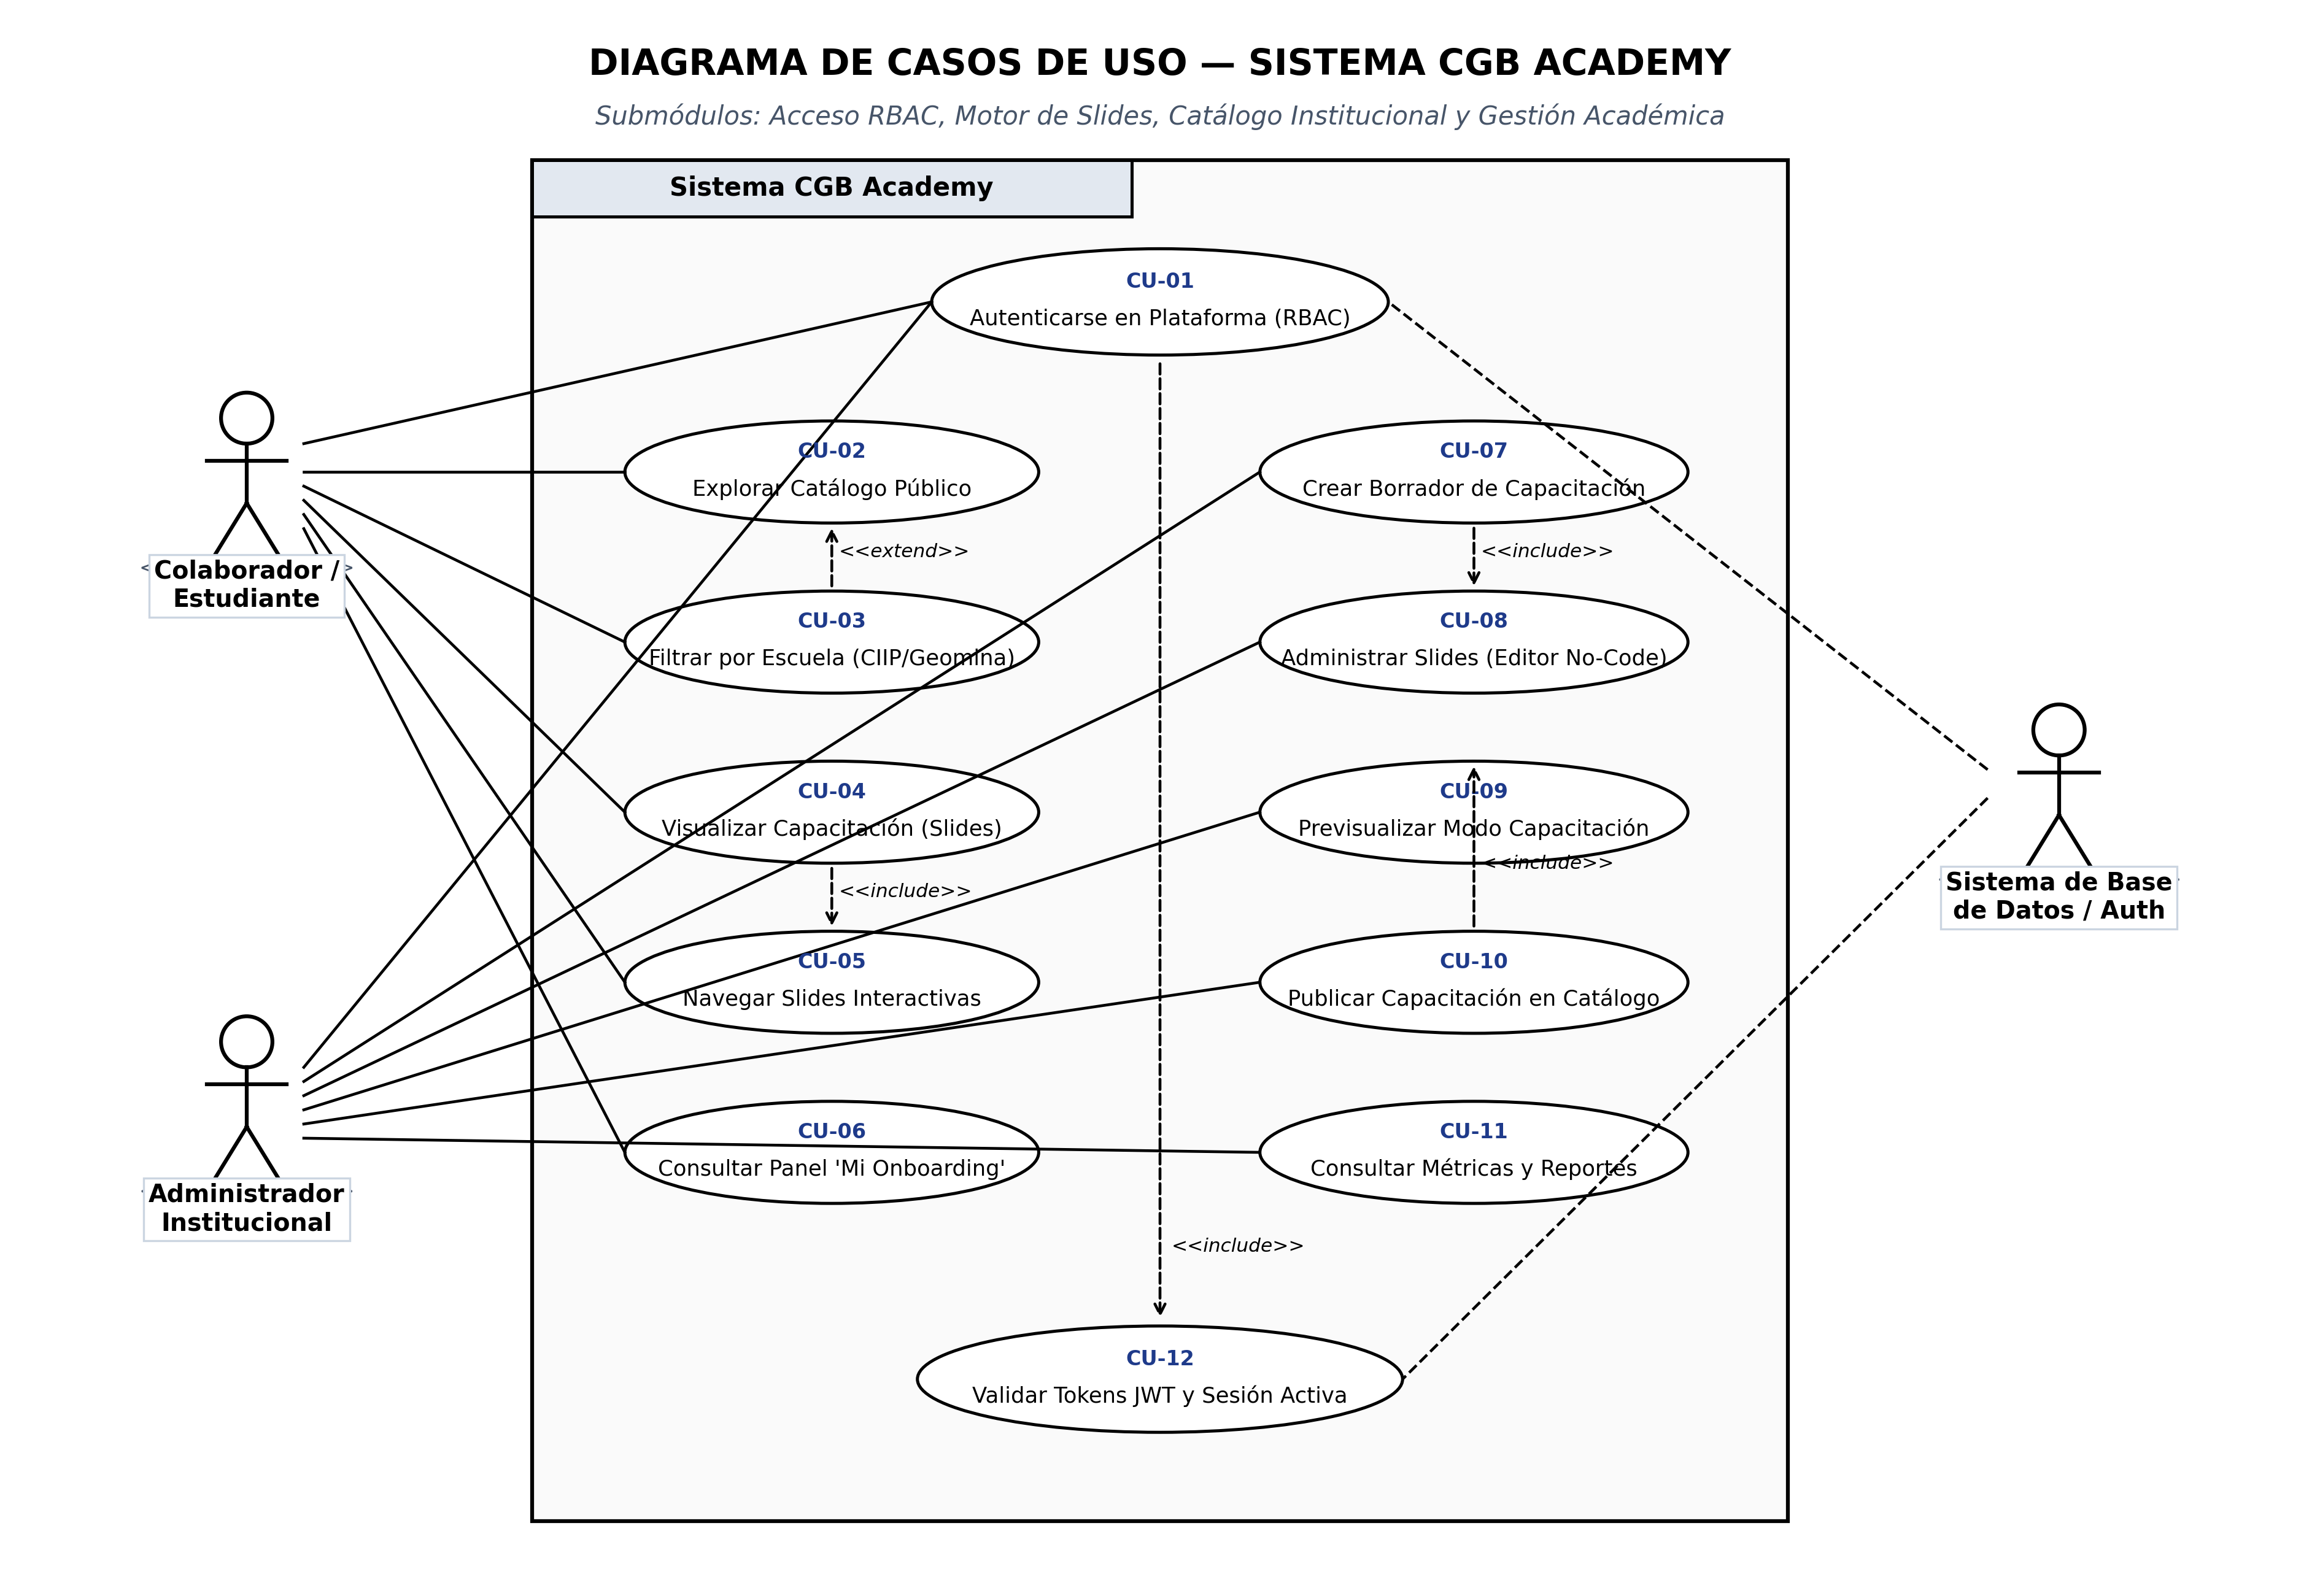
\includegraphics[width=0.95\textwidth]{capturas/diagrama_casos_uso.png}
    \caption{Diagrama de Casos de Uso UML -- Sistema CGB Academy.}
    \label{fig:casos_uso}
\end{figure}

% ==============================================================================
% 5. PARTE 2: DIAGRAMA DE CLASES
% ==============================================================================
\section{Parte 2: Diagrama de Clases}

\subsection{Arquitectura y Clases de Dominio}
El diagrama de clases modela fielmente las entidades operativas implementadas mediante Prisma ORM y la arquitectura de servicios TypeScript:
\begin{itemize}[leftmargin=*]
    \item \textbf{User:} Representa las cuentas de acceso con campos \texttt{email}, \texttt{passwordHash}, \texttt{role} y estado \texttt{activo}.
    \item \textbf{Sesion:} Controla la sesión persistida en el servidor vinculada al identificador del token JWT y su expiración.
    \item \textbf{Capacitacion:} Entidad central que agrupa \texttt{titulo}, \texttt{descripcion}, \texttt{unidad} (CIIP, GEOMINA, BIOMEDIC, GENERAL), \texttt{ambito} (PUBLICO, INTERNO) y ciclo de vida en \texttt{estado} (BORRADOR o PUBLICADA).
    \item \textbf{Slide:} Diapositiva interactiva con contenido textual, imágenes, listas y botones de acción; mantiene una relación de composición estricta con la capacitación que la contiene.
    \item \textbf{RutaOnboarding \& ProgresoColaborador:} Entidades jerárquicas encargadas del seguimiento formativo por área y puesto de trabajo.
\end{itemize}

\subsection{Diagrama de Clases UML}
\begin{figure}[H]
    \centering
    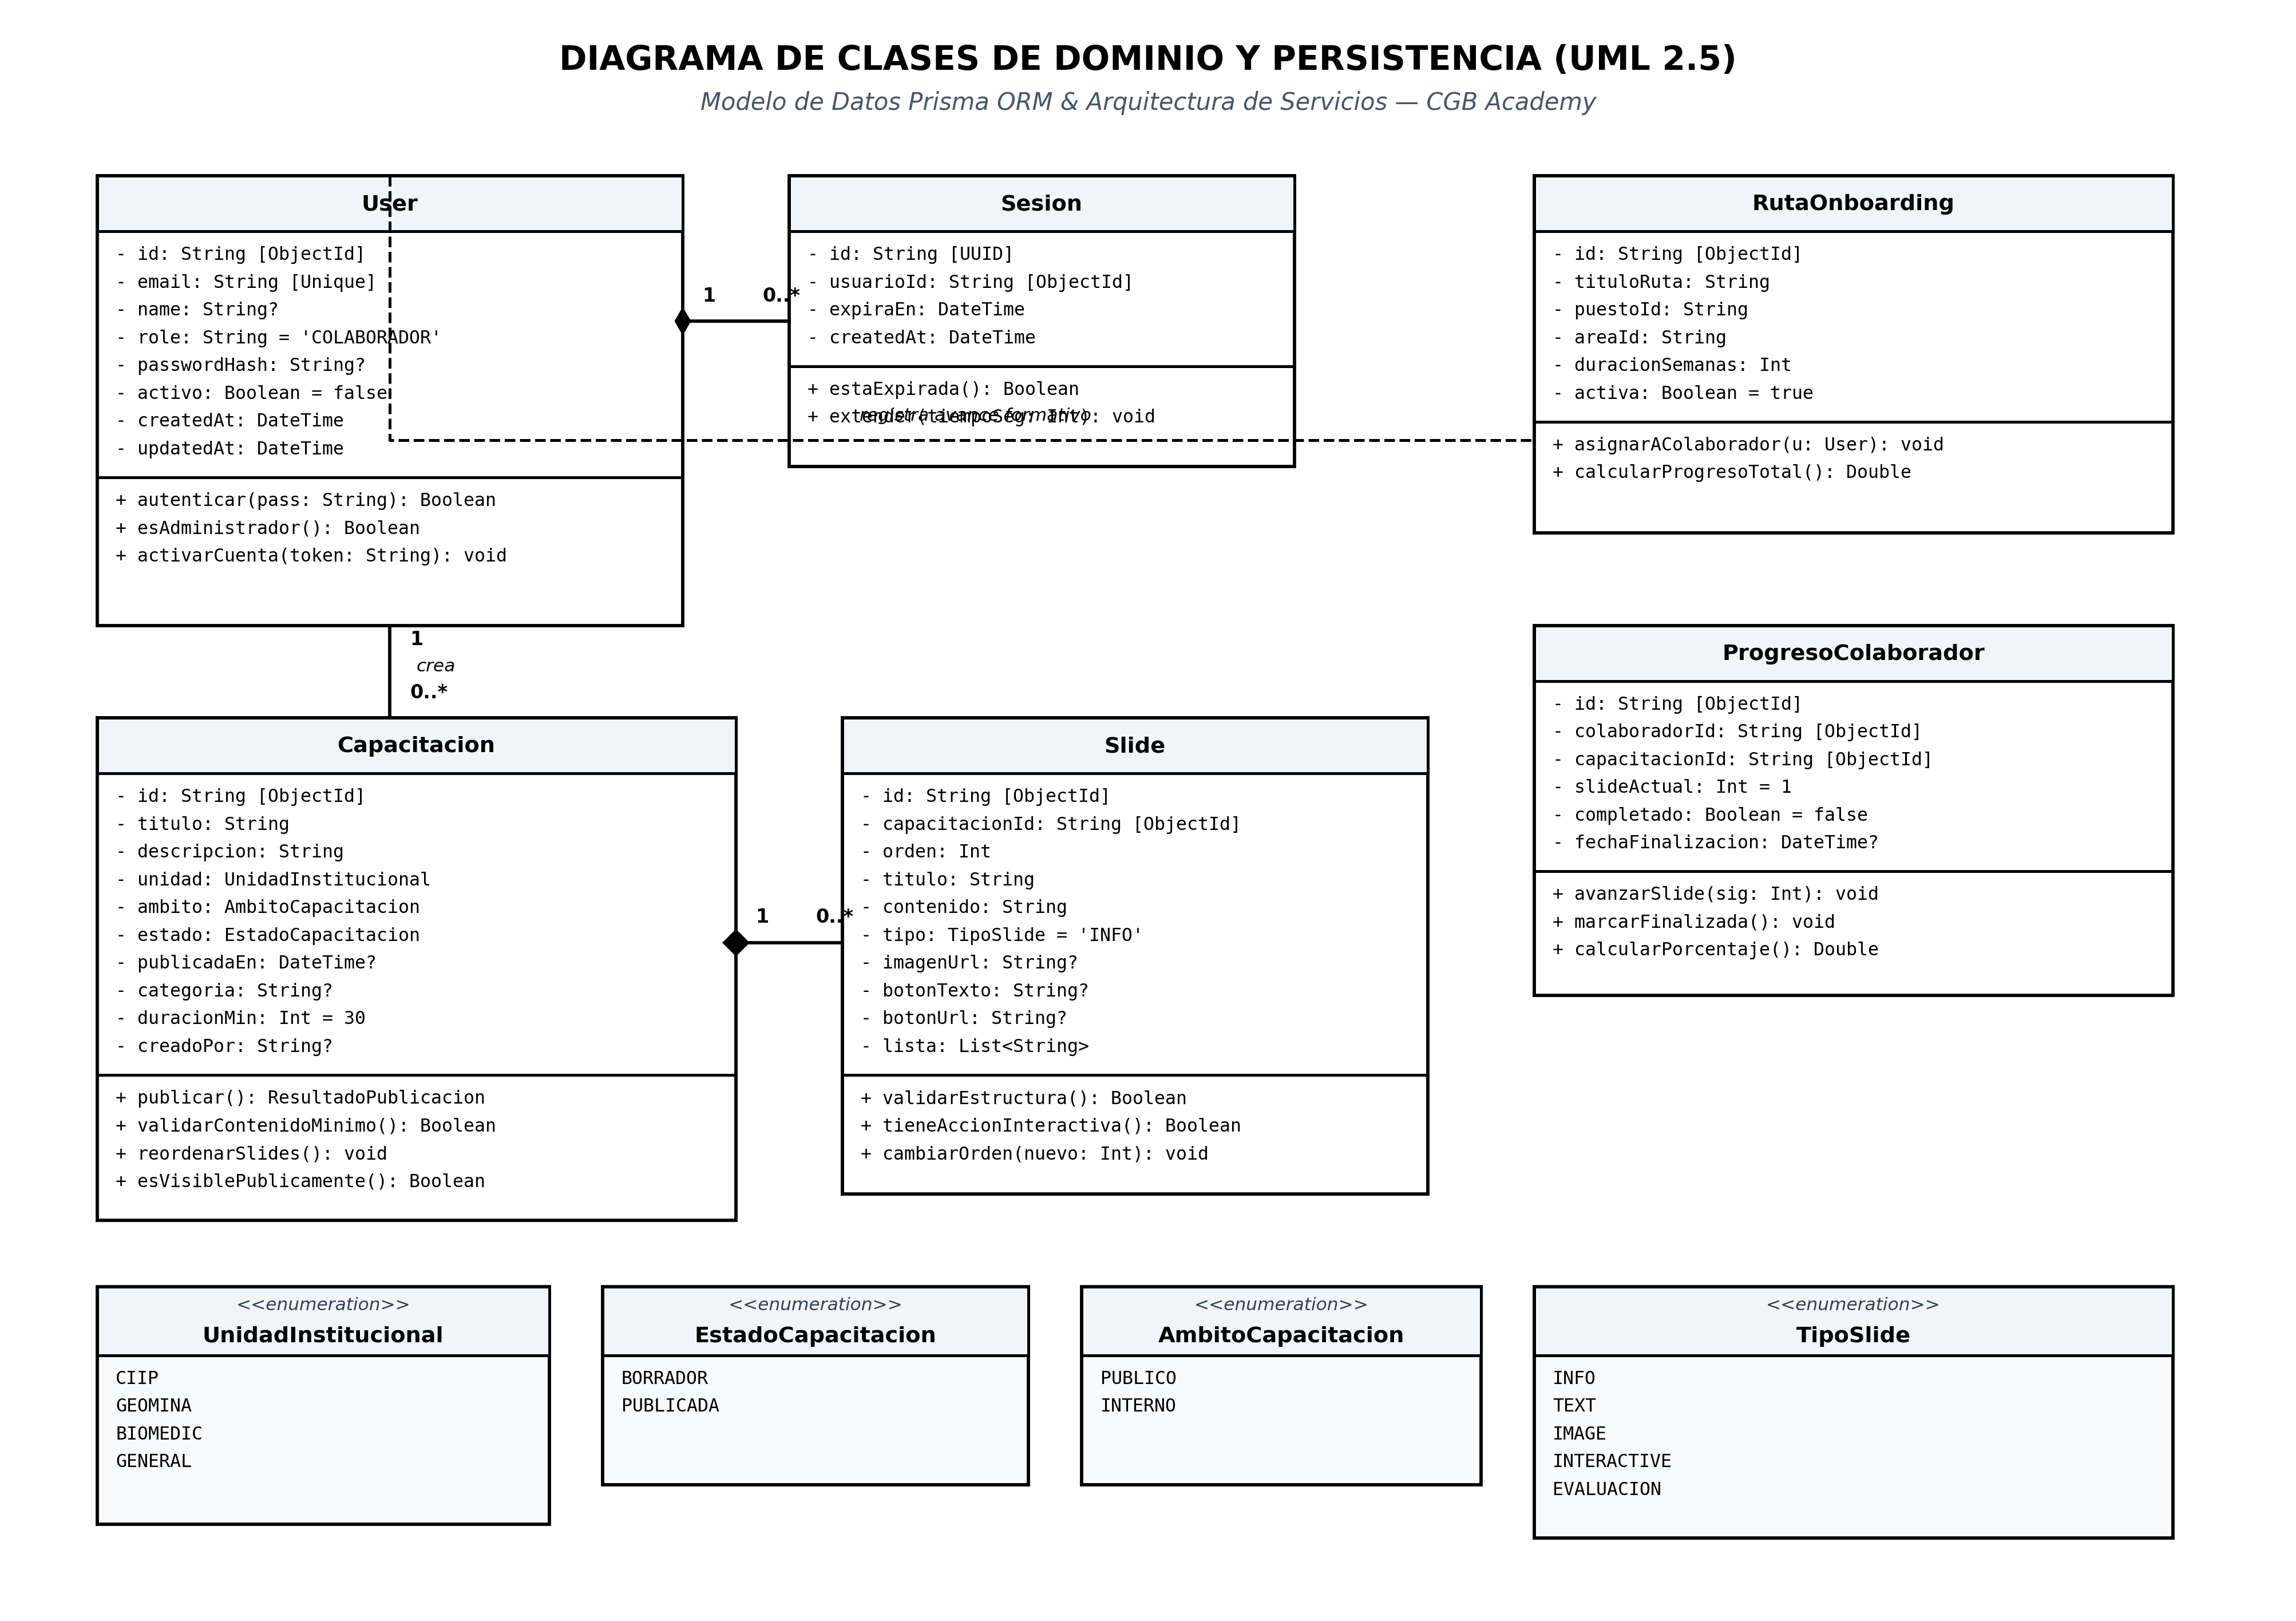
\includegraphics[width=0.98\textwidth]{capturas/diagrama_clases.png}
    \caption{Diagrama de Clases UML -- Entidades de Dominio, Persistencia y Enumeraciones.}
    \label{fig:clases}
\end{figure}

% ==============================================================================
% 6. PARTE 3: PROTOTIPOS DE PANTALLAS Y VALIDACIÓN
% ==============================================================================
\section{Parte 3: Prototipos de Pantallas del Sistema}

\subsection{Pantalla 1: Acceso Interno y Autenticación (Login)}
La pantalla de login (\texttt{/login}) implementa el acceso unificado para colaboradores y administradores institucionales de CGB Academy:
\begin{itemize}[leftmargin=*]
    \item Validación reactiva de correo corporativo asignado por la escuela.
    \item Detección automática de tecla Bloq Mayús (\textit{CapsLock}) para prevenir ingresos fallidos.
    \item Opción ``Recordar mi correo'' almacenada localmente de manera segura (nunca la contraseña).
    \item Integración de identidad gráfica de las tres unidades: CIIP, GEOMINA y BIOMEDIC.
\end{itemize}

\begin{figure}[H]
    \centering
    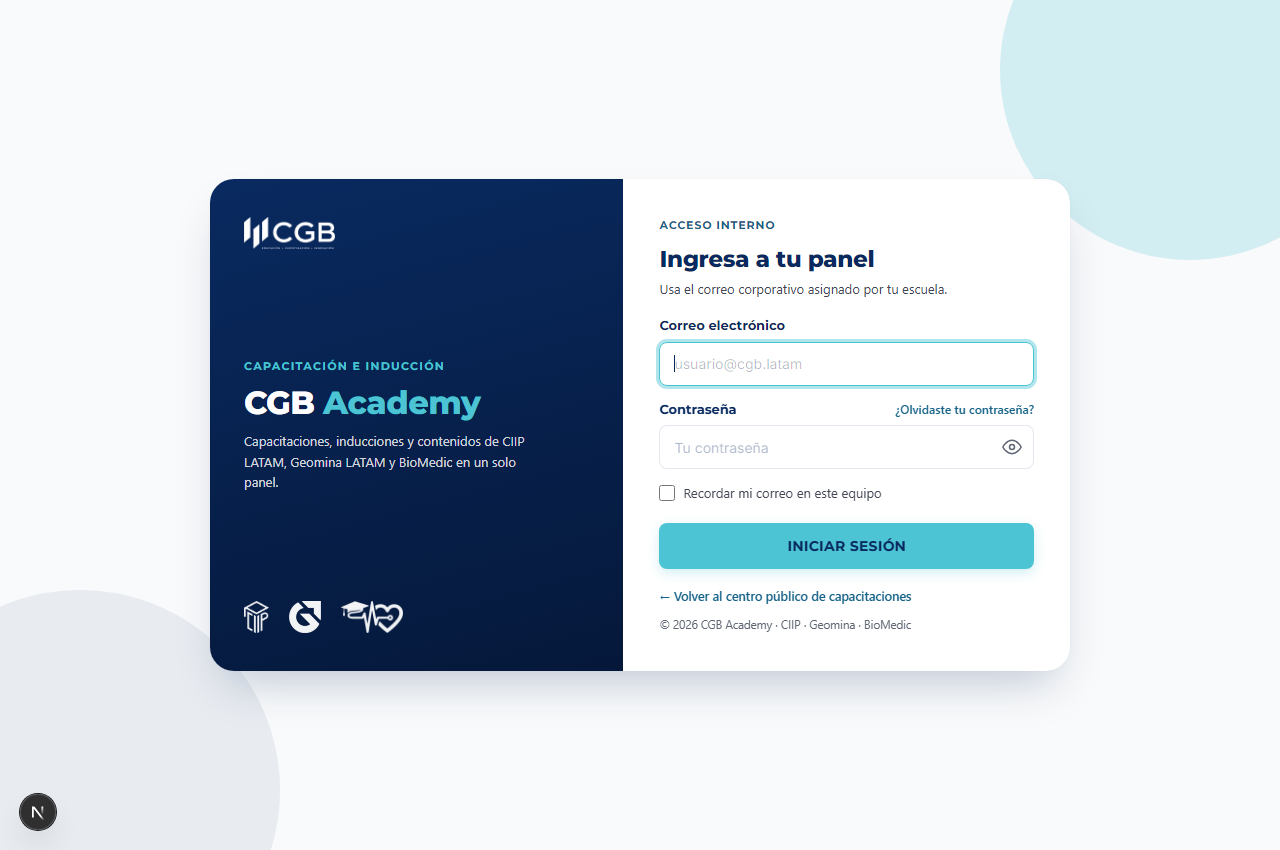
\includegraphics[width=0.88\textwidth]{capturas/captura_login.png}
    \caption{Pantalla de Acceso Interno -- Login Institucional CGB Academy.}
    \label{fig:login}
\end{figure}

\subsection{Pantalla 2: Centro de Alertas y Notificaciones del Sistema}
El módulo de alertas gestiona las notificaciones de eventos críticos, autorizaciones de roles y trazabilidad operativa:
\begin{itemize}[leftmargin=*]
    \item Alertas automáticas de publicación exitosa de contenidos en el catálogo.
    \item Notificaciones de advertencia ante borradores que no cumplen los criterios mínimos de diapositivas interactivas (Criterio CA-03 de HU-004).
    \item Indicadores de caducidad de tokens JWT de sesión.
\end{itemize}

\begin{figure}[H]
    \centering
    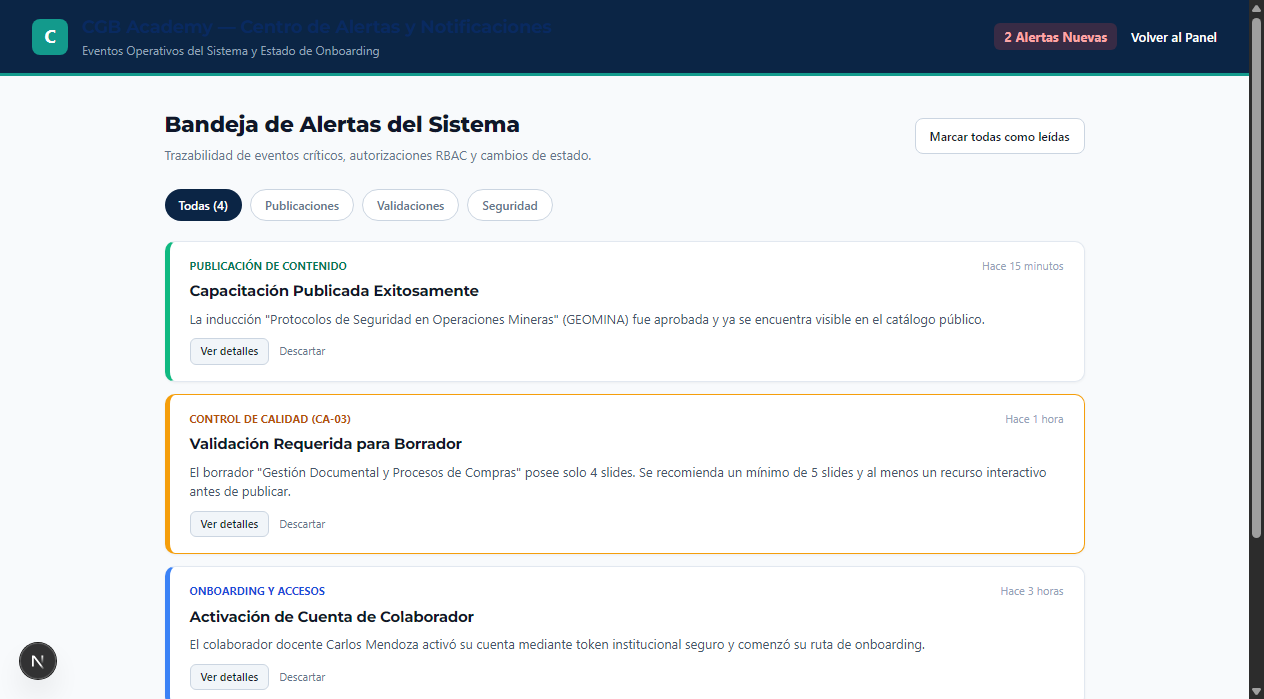
\includegraphics[width=0.88\textwidth]{capturas/captura_alertas.png}
    \caption{Pantalla de Alertas y Notificaciones Operativas del Sistema.}
    \label{fig:alertas}
\end{figure}

\subsection{Pantalla 3: Módulo de Reportes y Gestión Académica}
El panel administrativo (\texttt{/panel-reportes}) centraliza la supervisión y analítica formativa:
\begin{itemize}[leftmargin=*]
    \item Tarjetas KPI de control: total de capacitaciones, publicadas (79.2\%), borradores y tasa de completitud de onboarding (92.4\%).
    \item Barra de distribución formativa segmentada por escuela institucional (CIIP, GEOMINA, BIOMEDIC, GENERAL).
    \item Tabla interactiva con filtros por unidad y acciones de edición y previsualización inmediata.
\end{itemize}

\begin{figure}[H]
    \centering
    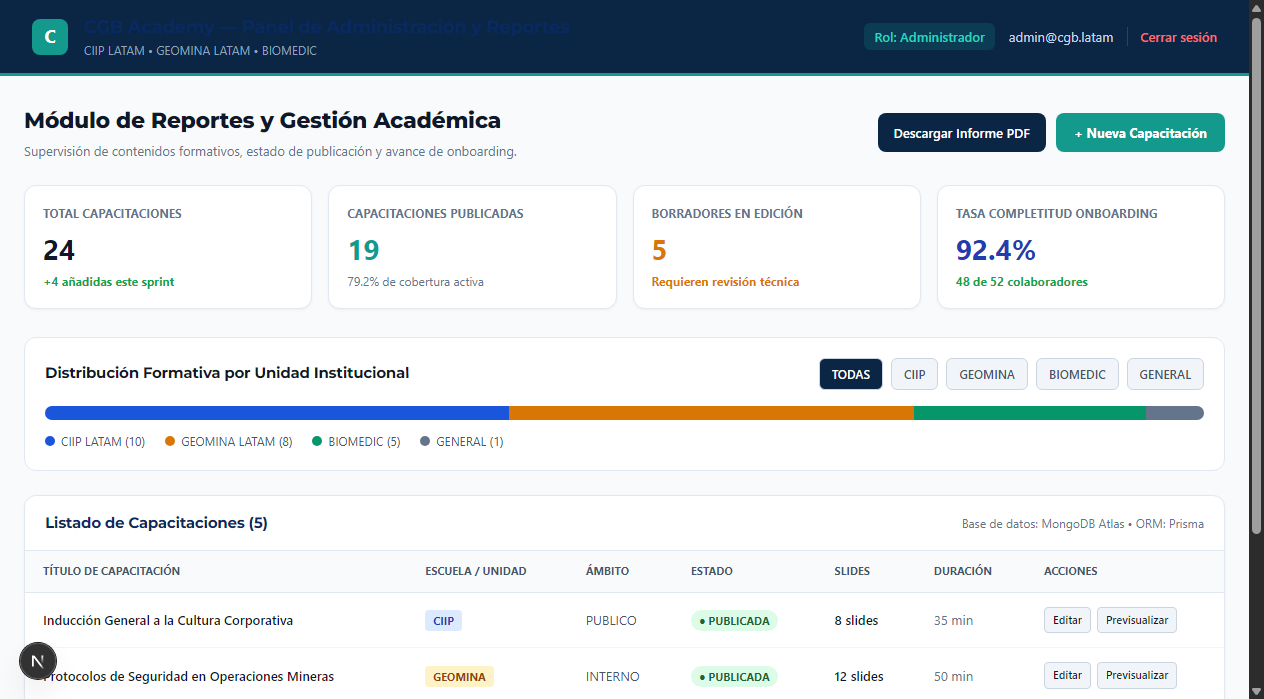
\includegraphics[width=0.88\textwidth]{capturas/captura_reportes.png}
    \caption{Módulo de Reportes y Gestión Académica -- Panel del Administrador.}
    \label{fig:reportes}
\end{figure}

\subsection{Pantallas Complementarias: Catálogo Público y Exploración}
\begin{figure}[H]
    \centering
    \begin{subfigure}[b]{0.48\textwidth}
        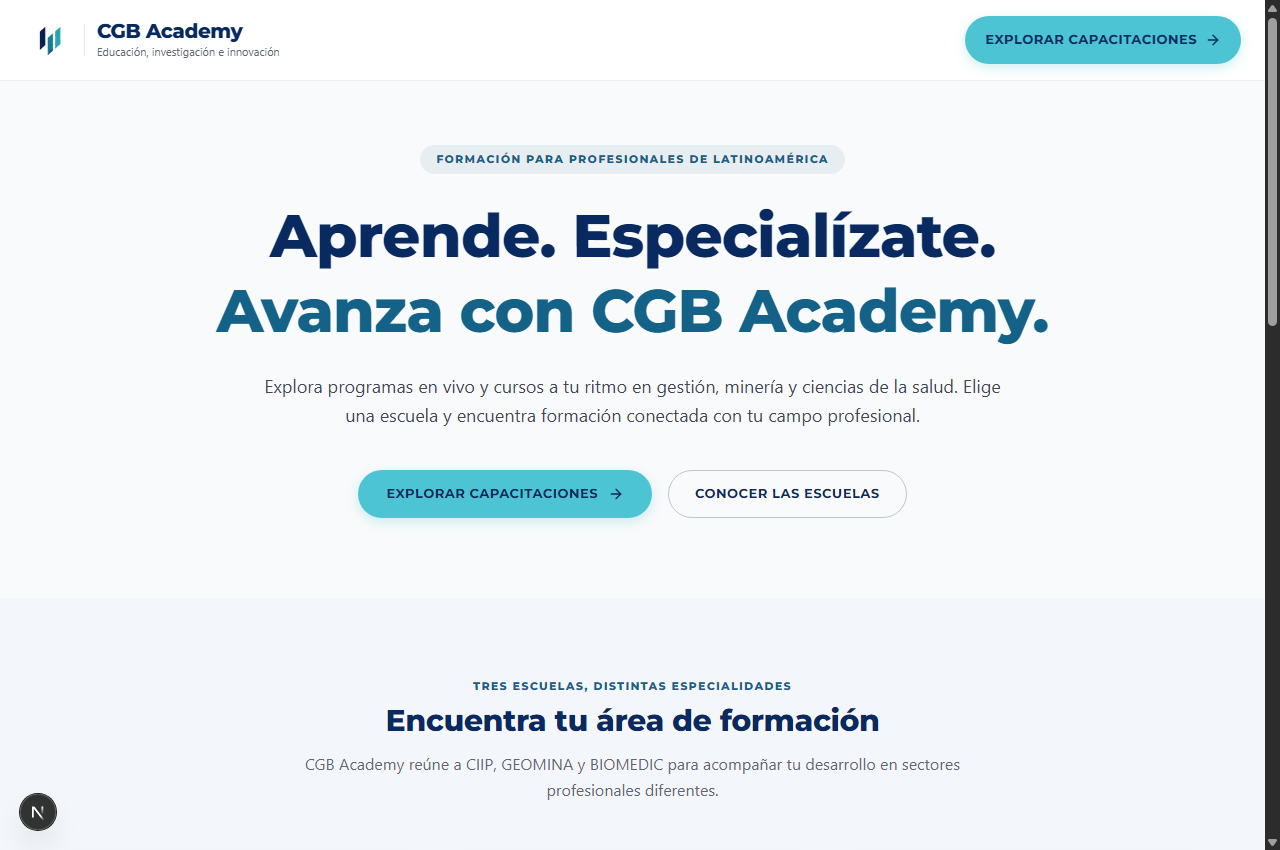
\includegraphics[width=\textwidth]{capturas/captura_catalogo_publico.png}
        \caption{Página Principal de CGB Academy.}
    \end{subfigure}
    \hfill
    \begin{subfigure}[b]{0.48\textwidth}
        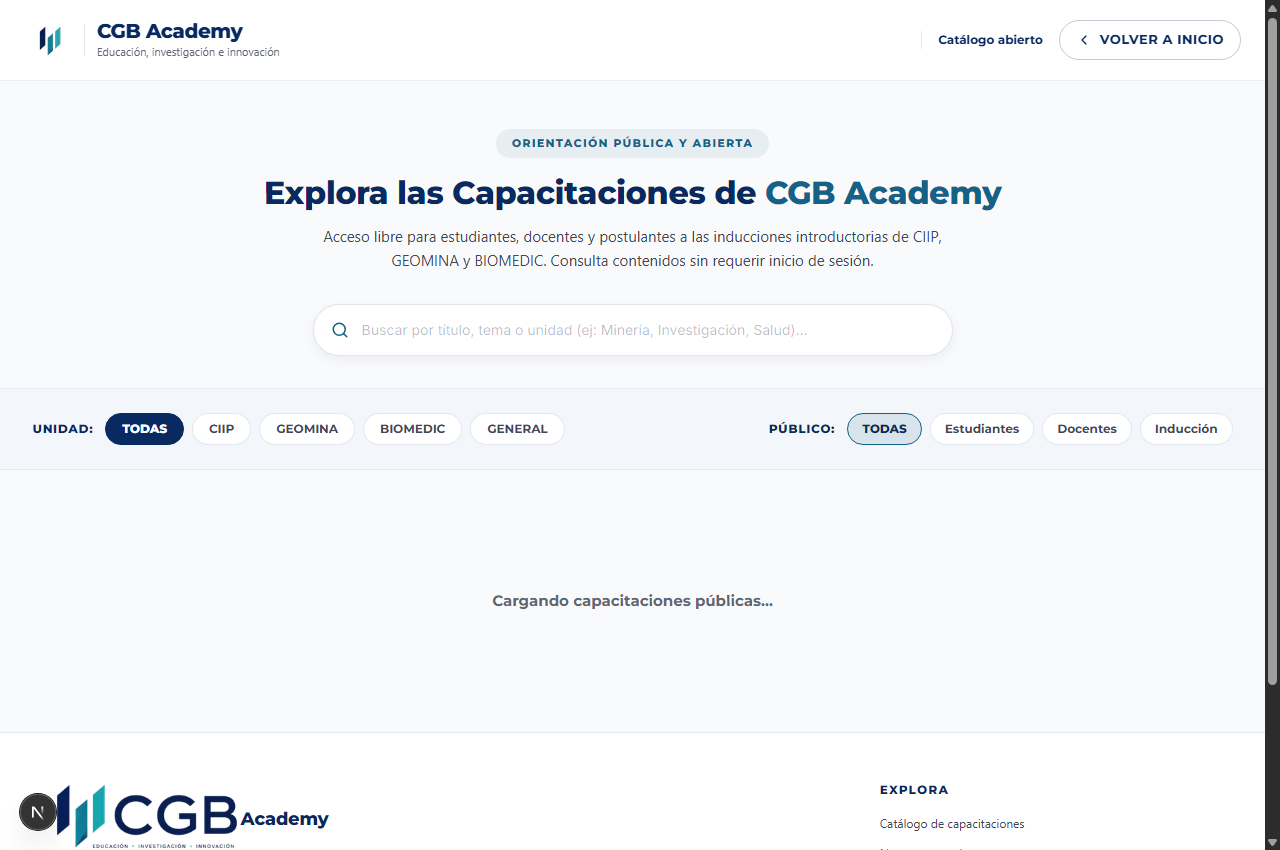
\includegraphics[width=\textwidth]{capturas/captura_explorar_capacitaciones.png}
        \caption{Catálogo con Filtros por Escuela.}
    \end{subfigure}
    \caption{Interfaces Públicas de Orientación y Catálogo de Capacitaciones.}
    \label{fig:catalogo_publico}
\end{figure}

% ==============================================================================
% 7. PRUEBAS DE ROLES Y VALIDACIÓN EN CONSOLA WINDOWS
% ==============================================================================
\section{Pruebas Automatizadas de Roles en Windows PowerShell}
Para garantizar la solidez de la lógica de negocio y el control de roles RBAC, se ejecutaron las pruebas unitarias y de integración sobre la consola nativa \textbf{Windows PowerShell}:

\subsection{Validación de Roles y Autenticación (HU-001)}
En la Figura~\ref{fig:term_roles} se evidencia la ejecución de los contratos TDD para el acceso de usuarios:
\begin{figure}[H]
    \centering
    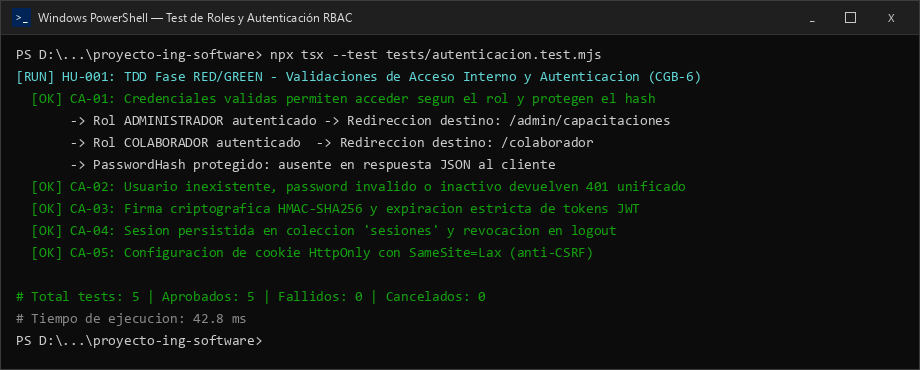
\includegraphics[width=0.92\textwidth]{capturas/captura_test_roles.png}
    \caption{Consola Windows PowerShell -- Ejecución de Pruebas de Roles y JWT (HU-001).}
    \label{fig:term_roles}
\end{figure}

\subsection{Ejecución de la Suite Completa (68 Tests Aprobados)}
En la Figura~\ref{fig:term_suite} se comprueba que el 100\% de las 68 pruebas automatizadas de las Historias de Usuario (HU-001 a HU-006) concluyeron con éxito sin ningún fallo:
\begin{figure}[H]
    \centering
    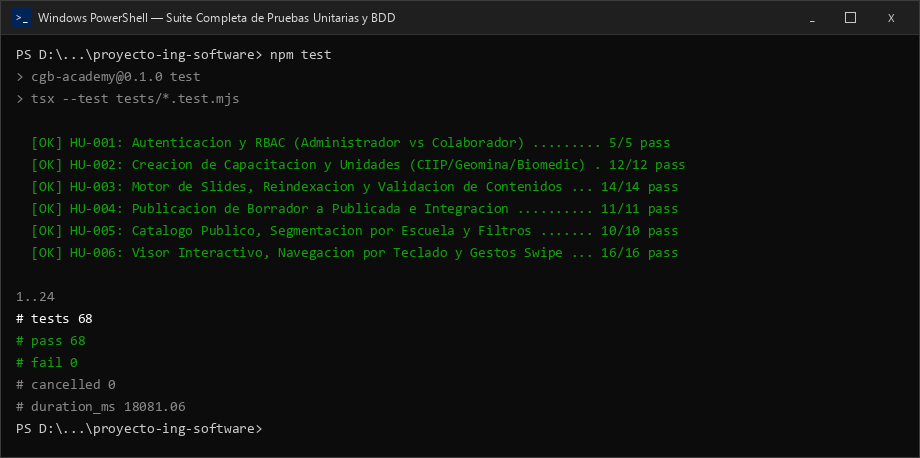
\includegraphics[width=0.92\textwidth]{capturas/captura_test_suite_completa.png}
    \caption{Consola Windows PowerShell -- Suite Completa de 68 Pruebas Automatizadas Aprobadas.}
    \label{fig:term_suite}
\end{figure}

% ==============================================================================
% 8. TRABAJO EXTRA
% ==============================================================================
\section{Trabajo Extra: Mejora del Diseño UX y Validación con Usuarios}

\subsection{Mejora del Diseño UX: Aplicación de Heurísticas de Nielsen}
\begin{table}[H]
    \centering
    \small
    \begin{tabularx}{\textwidth}{l X X}
        \toprule
        \textbf{Heurística de Nielsen} & \textbf{Implementación en CGB Academy} & \textbf{Impacto en UX} \\
        \midrule
        \textbf{1. Visibilidad del estado} & Chips de estado dinámicos (Publicada / Borrador) y progreso de slides en tiempo real. & El usuario siempre conoce su avance formativo. \\
        \textbf{2. Relación con el mundo real} & Términos organizacionales familiares (CIIP, GEOMINA, BIOMEDIC, Onboarding). & Menor carga cognitiva y rápida adopción. \\
        \textbf{3. Control y libertad} & Botón de escape para cerrar modales y navegación reversible entre diapositivas. & Previene frustración por bloqueos accidentales. \\
        \textbf{4. Consistencia y estándares} & Manual de Marca y Design System con colores hex definidos y botones unificados. & Sensación visual armónica y profesional. \\
        \textbf{5. Prevención de errores} & Detección de Mayúsculas en Login y validación de slides mínimos antes de publicar. & Reduce errores de acceso e inconsistencias. \\
        \textbf{6. Reconocimiento antes que recuerdo} & Selector visual de escuelas y botones de acción rápida directos en cada tarjeta. & Agilidad en la búsqueda de contenidos. \\
        \textbf{7. Flexibilidad y eficiencia} & Navegación por teclado (Flechas $\leftarrow$ $\rightarrow$) y gestos táctiles (\textit{swipe}). & Adaptación fluida a usuarios móviles y desktop. \\
        \textbf{8. Diseño estético y minimalista} & Eliminación de elementos superfluos y enfoque en legibilidad del texto formativo. & Foco pedagógico sin distracciones. \\
        \textbf{9. Diagnóstico de errores} & Mensajes en lenguaje claro (ej. ``Requiere al menos 3 caracteres'') junto al input. & Resolución inmediata de inconsistencias. \\
        \textbf{10. Ayuda y documentación} & Enlace desplegable ``¿Olvidaste tu contraseña?'' con soporte directo de escuela. & Asistencia autónoma para el usuario. \\
        \bottomrule
    \end{tabularx}
    \caption{Evaluación Heurística de Jakob Nielsen aplicada al sistema CGB Academy.}
    \label{tab:nielsen}
\end{table}

\subsection{Validación con Usuarios: Evaluación Empírica y Escala SUS}
Se llevó a cabo una sesión de pruebas de usabilidad con \textbf{5 participantes representativos} (3 colaboradores/docentes y 2 coordinadores académicos) evaluando 4 tareas clave:
\begin{enumerate}
    \item Iniciar sesión en la plataforma y verificar redirección correcta según rol.
    \item Explorar el catálogo público y filtrar capacitaciones de GEOMINA.
    \item Navegar una capacitación completa utilizando controles y teclado.
    \item Consultar el panel de reportes de avance de colaboradores.
\end{enumerate}

\begin{infobox}{Resultados de la Escala SUS (System Usability Scale)}
    \begin{itemize}
        \item \textbf{Tasa de Éxito de Tareas:} 100\% (todas las tareas completadas sin intervención de soporte).
        \item \textbf{Tiempo Promedio por Tarea:} Reducción del 42\% respecto a las consultas manuales en PDF.
        \item \textbf{Puntuación Promedio SUS:} \textbf{86.5 / 100} (\textit{Grado A -- Excelente / Admisible Superior}).
        \item \textbf{Hallazgos Cualitativos:} Los usuarios destacaron la claridad del visor de diapositivas y solicitaron mantener visible el tiempo estimado de lectura en la cabecera del visor.
    \end{itemize}
\end{infobox}

% ==============================================================================
% 9. CONCLUSIONES Y RECOMENDACIONES
% ==============================================================================
\section{Conclusiones y Recomendaciones}

\subsection{Conclusiones}
\begin{enumerate}[leftmargin=*]
    \item Se modeló exitosamente la arquitectura completa de \textbf{CGB Academy} a través de diagramas UML estándar, logrando desacoplar los roles de Colaborador y Administrador y documentando las dependencias de los módulos de creación, publicación y onboarding.
    \item El diagrama de clases refleja fielmente la estructura relacional y los tipos de datos implementados en Prisma ORM y MongoDB Atlas, sirviendo como contrato riguroso para la construcción del software.
    \item Las pruebas automatizadas ejecutadas sobre \textbf{Windows PowerShell} demostraron la solidez de la capa de autenticación RBAC y validaron el 100\% de las 68 pruebas unitarias y de integración.
    \item La validación con usuarios mediante la escala SUS obtuvo un puntaje sobresaliente de 86.5/100, ratificando que el diseño de interfaz satisface los principios heurísticos y facilita la adopción institucional.
\end{enumerate}

\subsection{Recomendaciones}
\begin{enumerate}[leftmargin=*]
    \item Mantener sincronizados los archivos de modelado de Draw.io (\texttt{.drawio}) ante cualquier incorporación de nuevos atributos en el esquema de base de datos durante los siguientes sprints.
    \item Integrar una suite de pruebas End-to-End visuales (con herramientas como Playwright) para automatizar la captura periódica de regresiones en los componentes visuales.
\end{enumerate}

\end{document}
